\documentclass[11pt]{article}
\usepackage[margin=1in]{geometry}
\usepackage{booktabs}
\usepackage{graphicx}
\usepackage{amsmath}
\usepackage{float}
\usepackage{hyperref}
\title{Descriptive Portfolio Analysis of Issued Loans}
\author{CO-KTU Workshop Credit Platform Data}
\date{Generated on 2026-06-08}

\begin{document}
\maketitle

\begin{abstract}
This report studies the 21,042 issued loans recorded in \texttt{export\_credits.csv}. The goal is descriptive rather than predictive: we summarize the platform's current operating condition, contractual revenue base, available loss and exposure indicators, expected contractual cash flows for unresolved loans, and credit performance. Customer-level application flow is used only to motivate the transition into the issued-loan portfolio; all portfolio analysis after issuance uses loan identifiers.
\end{abstract}

\section{Scope and Unit of Analysis}
The full data funnel contains 34,201 registered customers, of whom 26,289 have loan application evidence. A customer may appear in both rejected and approved paths. The approved path contains 8,046 unique customers, consisting of 2,050 customers with issued credit and no rejection rows plus 5,996 customers with both rejection history and issued credit. These 8,046 customers account for 21,042 issued loans. The rejected-application table contains 64,039 rejected application rows, but rejected loans are outside the main analytical scope of this report.

\begin{figure}[H]
\centering
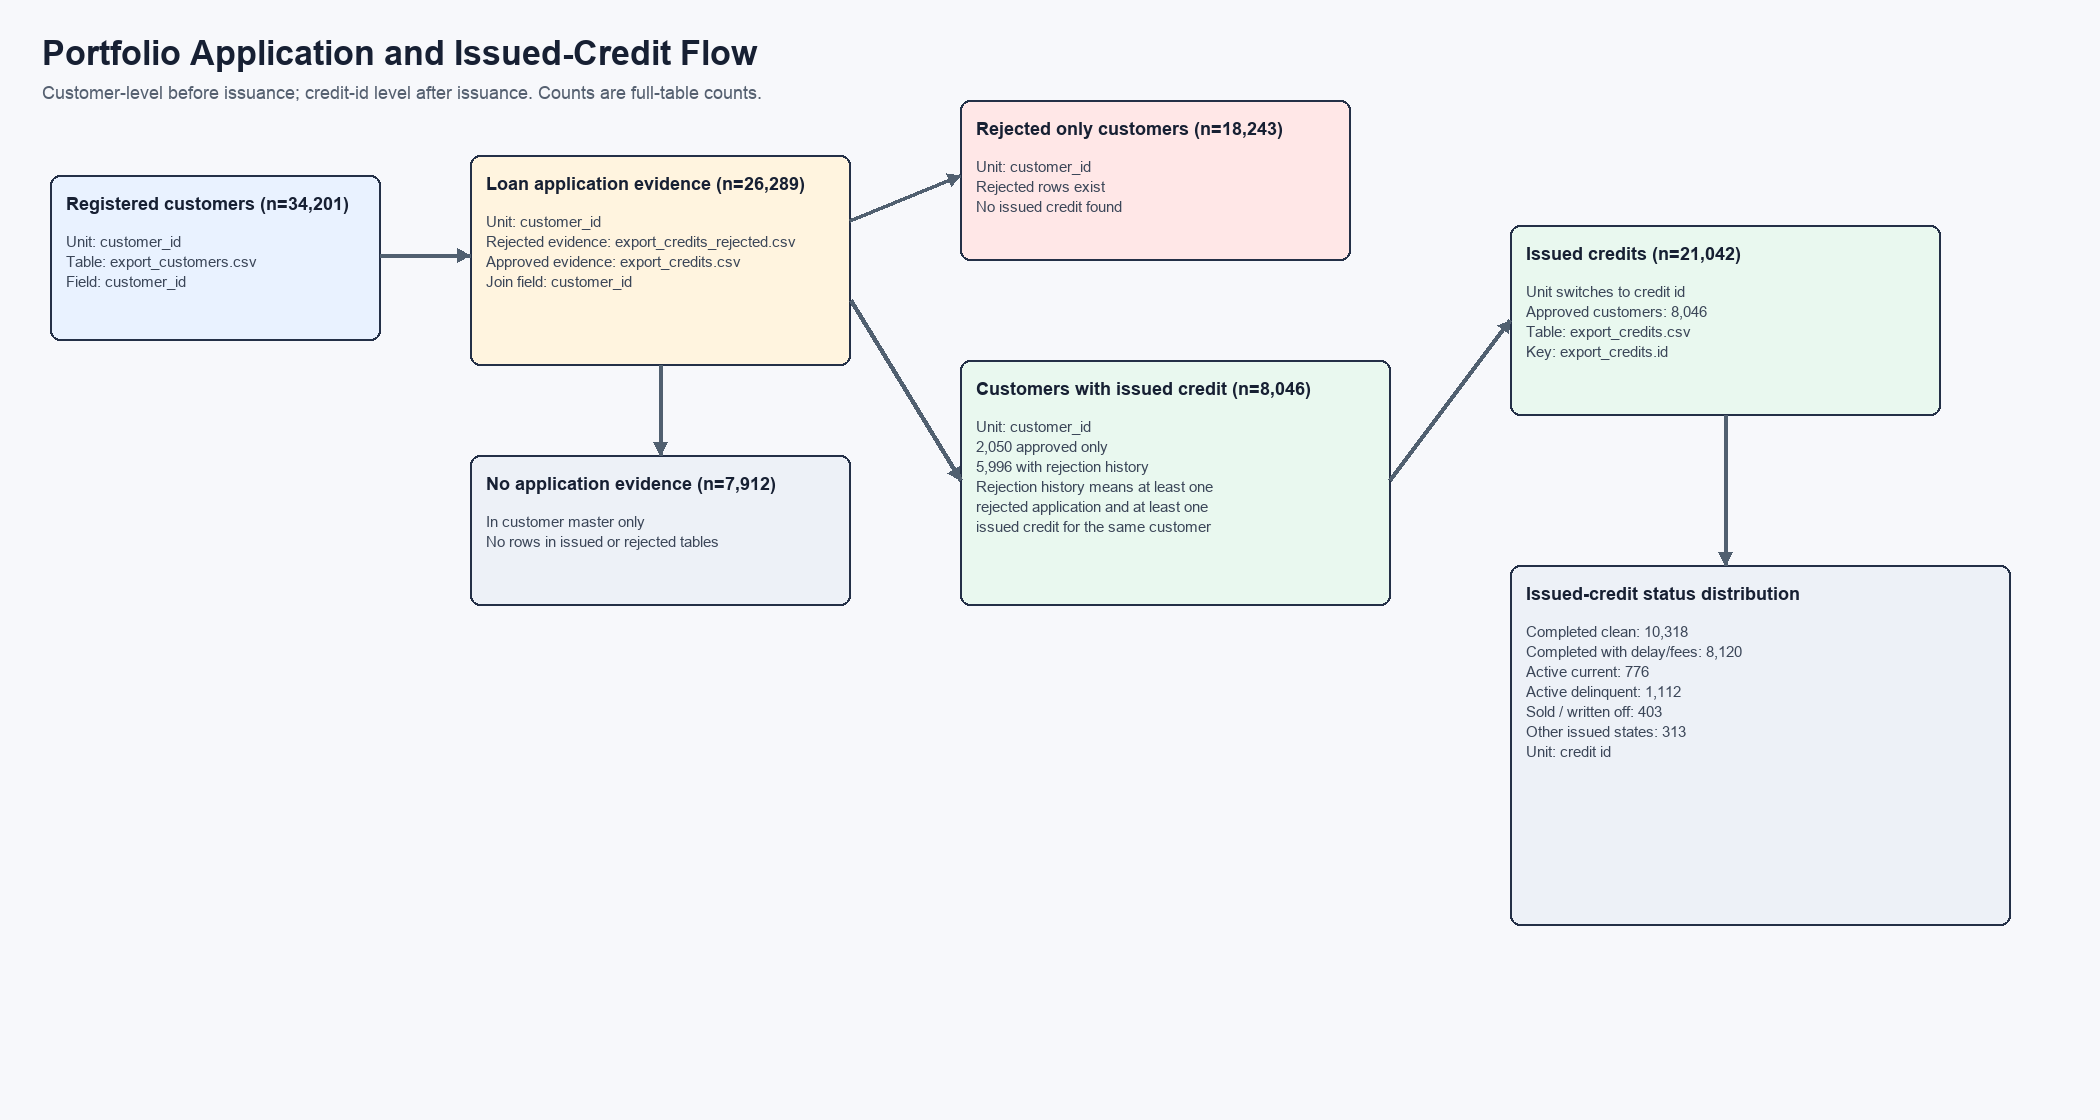
\includegraphics[width=0.95\linewidth]{portfolio_flowchart.png}
\caption{Portfolio funnel. Customer-level counts are used before issuance; credit-id level counts are used after issuance.}
\end{figure}

The unit of analysis is therefore the issued loan:
\[
i \in \{1,\ldots,N\}, \quad N = 21,042.
\]
Completed loans are identified by a non-empty \texttt{paid} field. Ongoing loans are those with an empty \texttt{paid} field. Because actual payment transaction records are not available, monetary revenue measures should be interpreted as contractual or proxy measures, not audited cash receipts.

\section{Definitions and Formulas}
For loan \(i\), let \(A_i\) denote principal amount, \(C_i\) contractual charge, \(F_i\) late fee balance, and \(X_i\) completed extension request fees. The contractual revenue proxy is
\[
R_i^{contract} = C_i + F_i + X_i.
\]
For completed loans with \texttt{paid} present and zero remaining debt, the completed-loan gross revenue proxy is
\[
R_i^{completed} = C_i + F_i + X_i.
\]
This assumes that loan completion implies collection of scheduled contractual charges. It is an assumption imposed by data limitations, because individual cash payment transactions are not observed.

Remaining exposure is defined as
\[
E_i = \max(\texttt{debt}_i, \texttt{s\_debt}_i, \texttt{r\_debt}_i).
\]
High-risk or impaired exposure is the sum of \(E_i\) over loans classified as currently delinquent, sold/written off, or unpaid past maturity. This is an exposure proxy, not a realized accounting loss.

\section{Portfolio Overview}
The issued portfolio contains 21,042 loans to 8,046 borrowers. Total issued principal is EUR 27,231,984.90. The average loan amount is EUR 1,294.17, and the median is EUR 800.00. The average contractual period is 677.4 days, with a median of 720 days.

\begin{figure}[H]
\centering
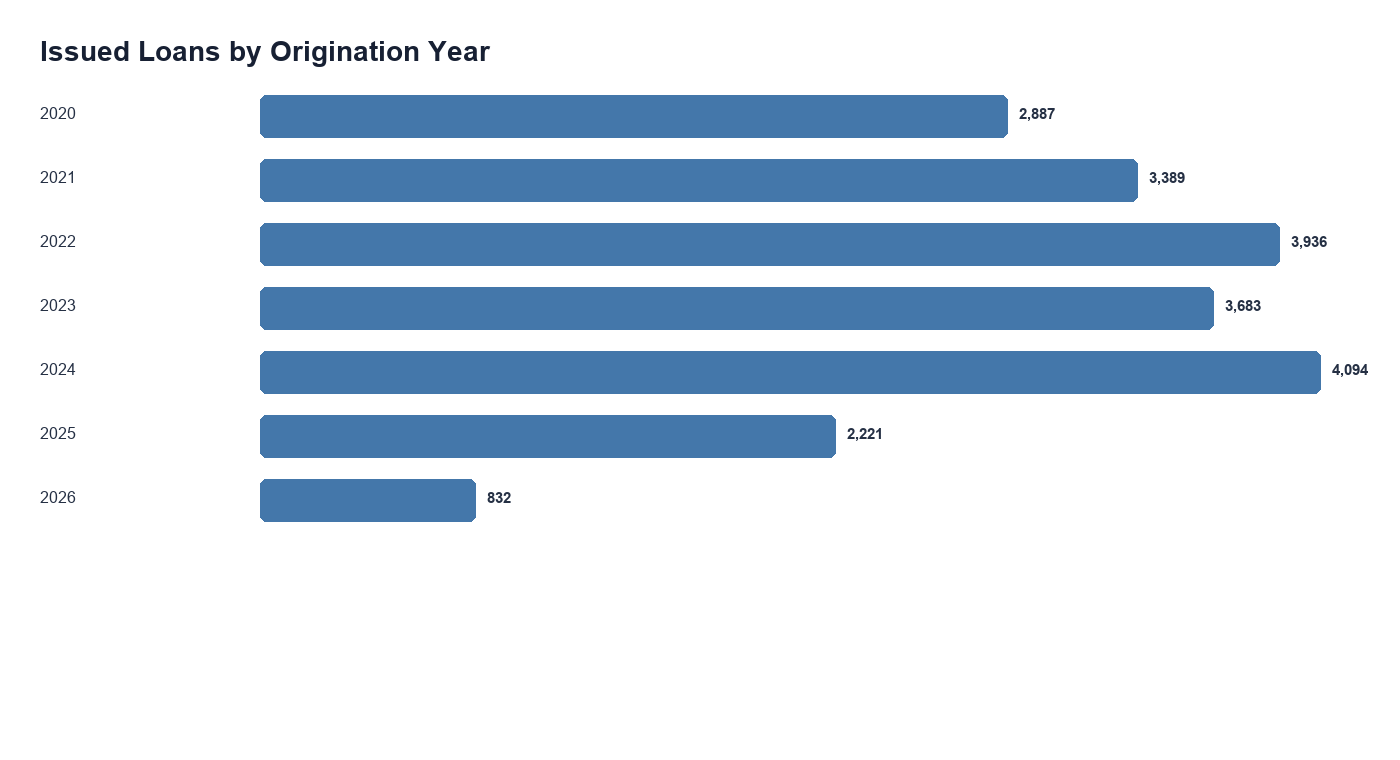
\includegraphics[width=0.85\linewidth]{annual_issued_loans.png}
\caption{Issued loans by origination year.}
\end{figure}

\section{Revenue Analysis}
The revenue analysis is based on fields available in the issued-loan table and extension-request table. The main planned revenue field is \texttt{charge}, which largely decomposes into interest and administrative fees. Late fees and completed extension request fees are reported separately.

\begin{table}[H]
\centering
\caption{Revenue-related measures. Values are contractual/proxy measures, not audited cash receipts.}
\begin{tabular}{lr}
\toprule
Metric & EUR \\
\midrule
Contractual charge & 23,132,792.39 \\
Administrative fee component & 10,590,067.19 \\
Interest component & 12,539,558.43 \\
Insurance component & 0.00 \\
Late fee balance & 39,566.39 \\
Completed extension request fees & 879,291.09 \\
Completed-loan gross revenue proxy & 19,339,345.85 \\
\bottomrule
\end{tabular}
\end{table}

The completed-loan gross revenue proxy is EUR 19,339,345.85. This measure includes only loans that are marked paid and have zero remaining debt. It excludes unresolved loans because their final cash outcome is not yet observed.

\section{Cost and Loss Analysis}
The available data do not include funding cost, acquisition cost, servicing cost, or recovery proceeds from sold debt. Therefore, the analysis focuses on credit exposure and loss proxies rather than full cost accounting. Total remaining exposure, defined by \(E_i\), is EUR 4,751,059.43. High-risk or impaired exposure is EUR 2,385,072.97. Active-current exposure is EUR 2,365,986.46.

These figures should be interpreted as portfolio risk indicators. They do not prove realized loss, especially for active delinquent loans that may later cure or be recovered.

\section{Expected Contractual Cash Flow for Ongoing Loans}
The schedule table \texttt{credits\_schedules\_all.csv} provides planned installment dates and amounts. For unresolved loans, expected future scheduled receipts are computed as:
\[
\text{FutureScheduled} = \sum_{i: \texttt{paid}_i=\emptyset} \sum_{t \geq 2026-06-08} \texttt{pay\_sum}_{i,t}.
\]
This is a contractual schedule measure. It is not a forecast of actual repayment behavior.

Among issued loans, 12,859 have schedule rows in the current schedule export. For ongoing loans covered by schedules, future scheduled receipts from 2026-06-08 onward total EUR 54,513.79, composed of EUR 32,337.40 principal, EUR 2,814.39 interest, and EUR 19,362.00 administrative fee.

\begin{figure}[H]
\centering
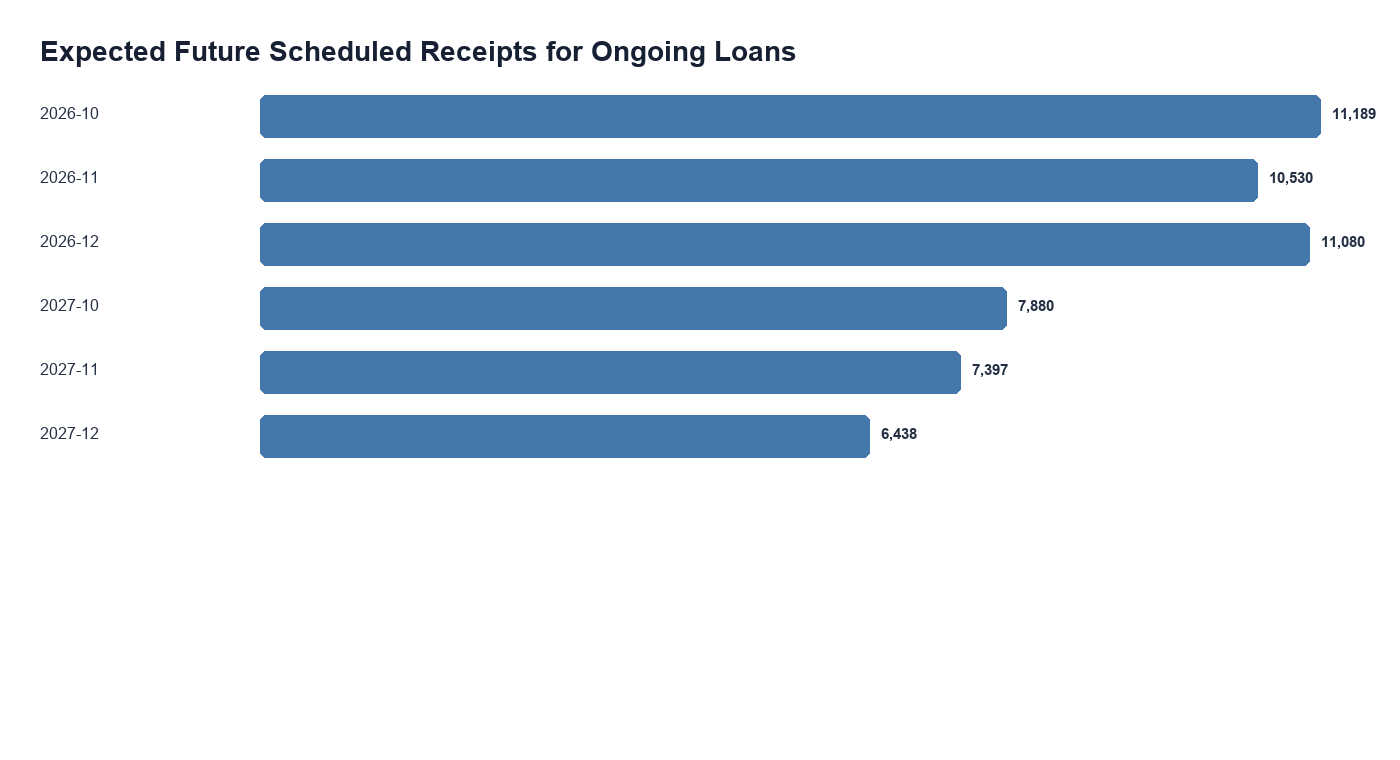
\includegraphics[width=0.9\linewidth]{expected_future_schedule_cashflow.png}
\caption{Expected future scheduled receipts for unresolved loans, grouped by planned pay month.}
\end{figure}

\section{Credit Performance and Risk}
Credit performance is summarized using status classifications derived from \texttt{paid}, remaining debt fields, current and maximum delay, late fees, sold flags, and writeoff fields.

\begin{table}[H]
\centering
\caption{Issued-credit status distribution.}
\begin{tabular}{lrrrr}
\toprule
Status & Loans & Share & Principal & Outstanding exposure \\
\midrule
Completed clean & 10,318 & 49.0\% & 12,662,201.78 & 0.00 \\
Completed with delay/fees & 8,120 & 38.6\% & 8,672,219.54 & 0.00 \\
Active delinquent & 1,112 & 5.3\% & 2,167,632.83 & 1,939,056.80 \\
Active current & 776 & 3.7\% & 1,902,143.48 & 2,365,986.46 \\
Sold / written off & 403 & 1.9\% & 386,512.54 & 445,081.67 \\
Other unpaid/no debt & 309 & 1.5\% & 1,437,108.00 & 0.00 \\
Unpaid past maturity & 4 & 0.0\% & 4,166.73 & 934.50 \\
\bottomrule
\end{tabular}
\end{table}

\begin{figure}[H]
\centering
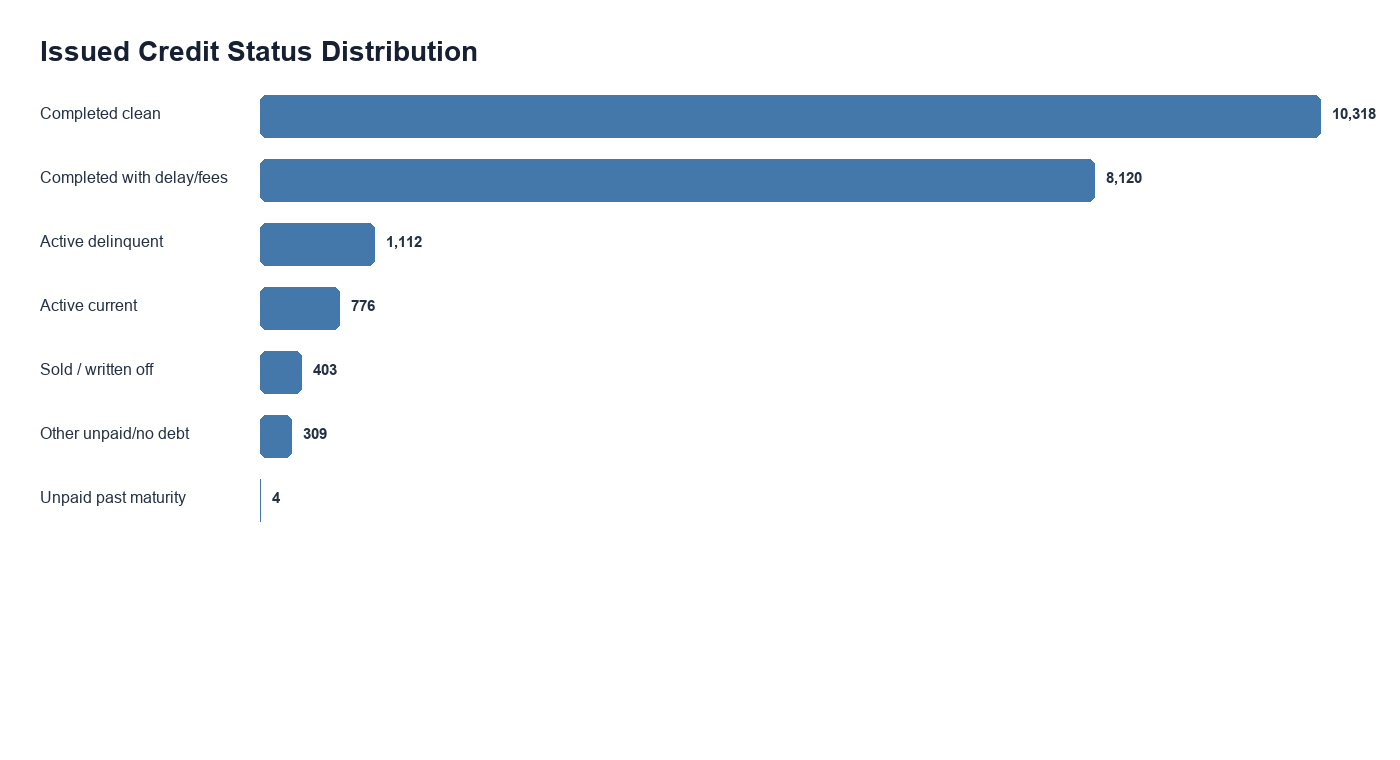
\includegraphics[width=0.85\linewidth]{issued_status_distribution.png}
\caption{Issued-credit status distribution.}
\end{figure}

Historical delinquency is represented by \texttt{max\_delay}, while current delinquency is represented by \texttt{current\_delay}.

\begin{table}[H]
\centering
\caption{Historical maximum delay buckets.}
\begin{tabular}{lrr}
\toprule
Bucket & Loans & Share \\
\midrule
0 & 10,924 & 51.9\% \\
1-30 & 7,194 & 34.2\% \\
31-60 & 439 & 2.1\% \\
61-90 & 220 & 1.0\% \\
90+ & 2,265 & 10.8\% \\
\bottomrule
\end{tabular}
\end{table}

\begin{table}[H]
\centering
\caption{Current delay buckets.}
\begin{tabular}{lrr}
\toprule
Bucket & Loans & Share \\
\midrule
0 & 11,712 & 55.7\% \\
1-30 & 6,819 & 32.4\% \\
31-60 & 410 & 1.9\% \\
61-90 & 201 & 1.0\% \\
90+ & 1,900 & 9.0\% \\
\bottomrule
\end{tabular}
\end{table}

The portfolio has 10,318 cleanly completed loans and 8,120 completed loans with delay or fee signals. There are 1,112 currently delinquent active loans and 403 sold or written-off loans.

\section{Conclusion}
The issued portfolio is large enough for descriptive operating analysis: 21,042 issued loans, EUR 27,231,984.90 in principal, and EUR 23,132,792.39 in contractual charges. The data support portfolio overview, contractual revenue analysis, credit exposure analysis, expected contractual cash-flow analysis for unresolved loans, and credit performance analysis.

However, the available data do not contain actual installment-level payment transactions. Therefore, profitability is evaluated as a contractual and credit-risk proxy. A definitive accounting profit statement would require actual cash collections, funding cost, operating cost, acquisition cost, and recovery proceeds.

\end{document}
